\begin{figure}[t]
    \centering
    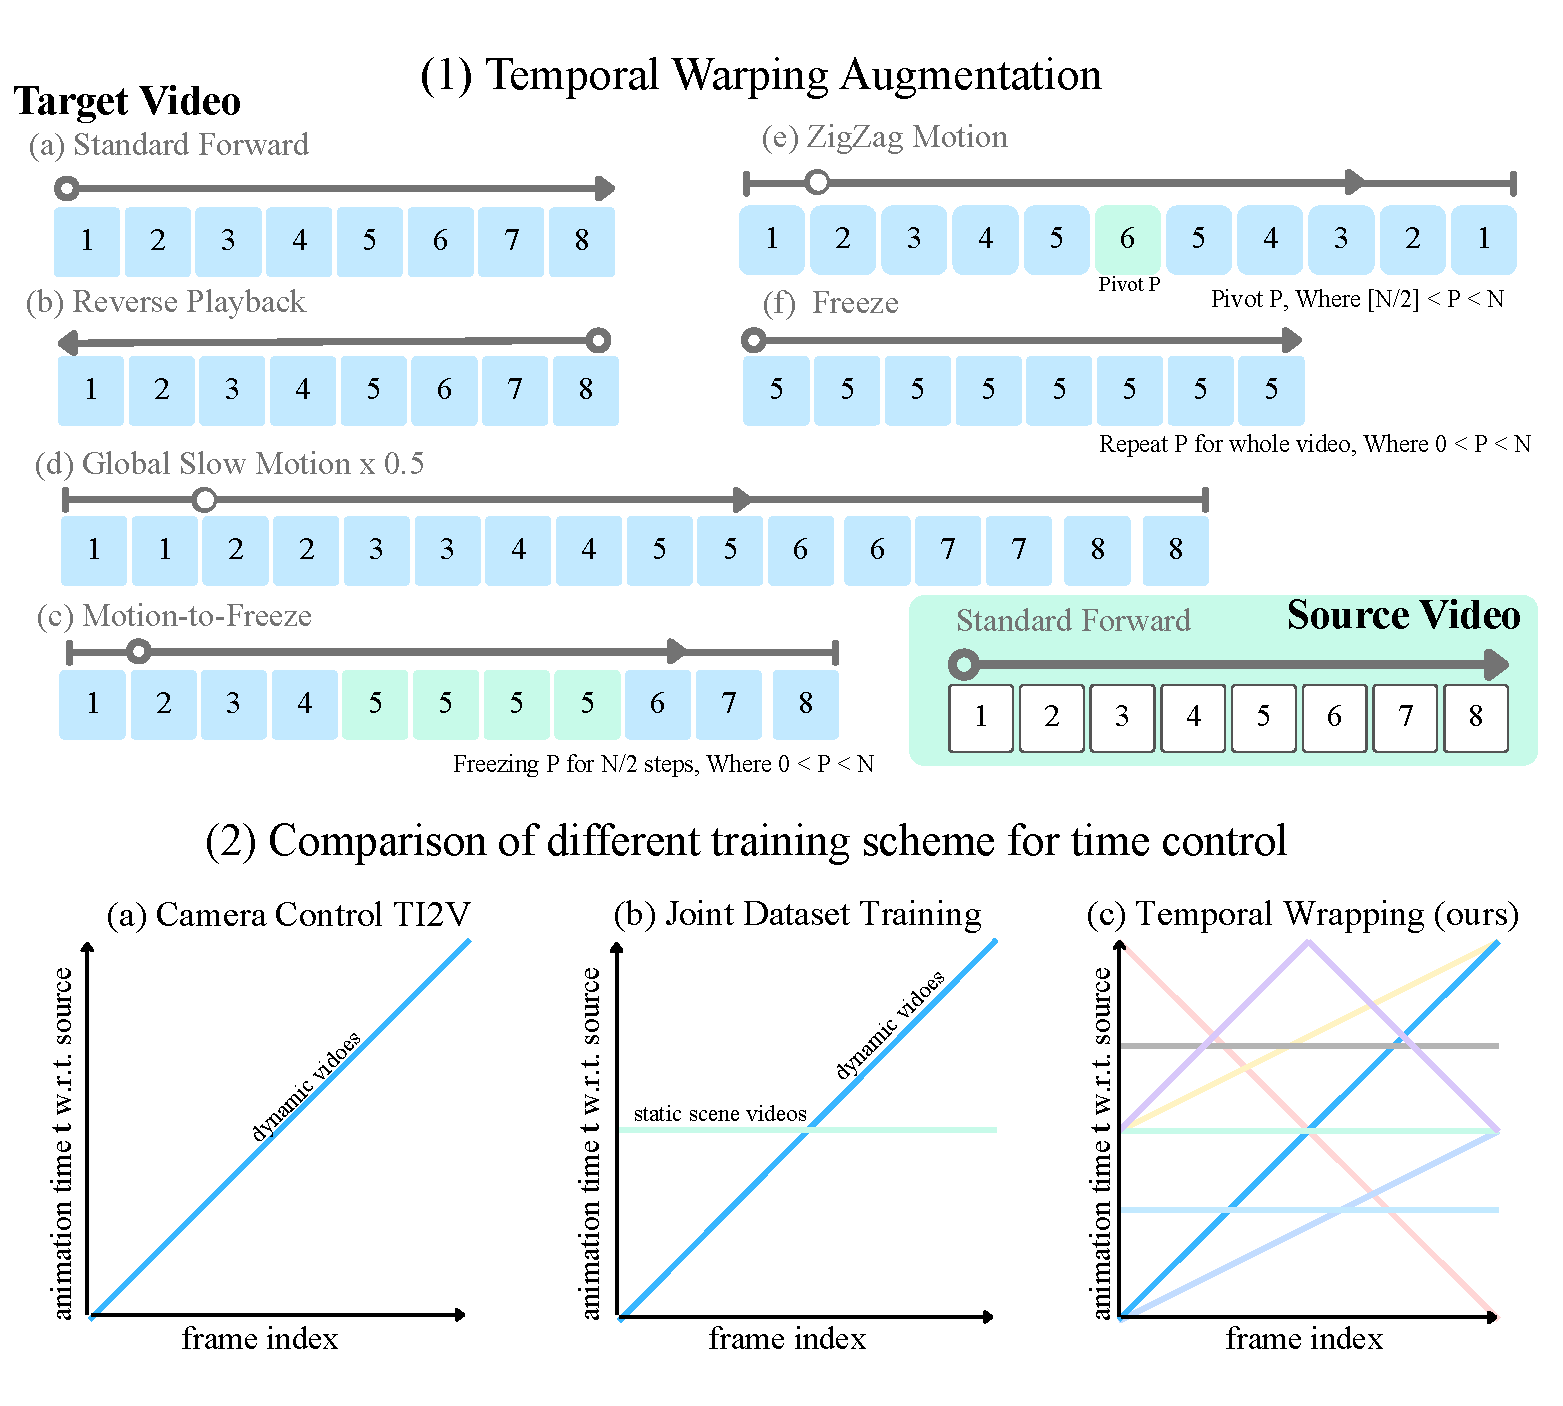
\includegraphics[width=\linewidth]{figures/src_files/TWA.pdf}
    \vspace{-0.5cm}
    \caption{
        \textbf{Temporal Wrapping for Spatiotemporal Disentanglement.}
        (Top) For multi-view dynamic scene datasets \cite{Bai2025}, a set of temporal warping operations (e.g.\, reverse playback, zigzag motion, slow motion, and freeze) are applied to the target video, with the source video kept as the standard forward reference, providing explicit supervision for temporal control  .
        (Bottom) Compared with existing camera-control \cite{vanhoorick2024gcd, Bai2025} and joint-dataset training strategies \cite{Wu2024, watson2025controllingspacetimediffusion}, which rely on monotonic time progression and static-scene videos to demonstrate temporal differences, Temporal Wrapping provide much more diverse and explicit signals of temporal variation, leading to disentanglement of space and time.
    }
    \label{fig:temporal_wrapping}
    \vspace{-0.3cm}
\end{figure}


(Top) For multi-view dynamic scene datasets, a set of temporal warping operations, including reverse, playback, zigzag motion, slow motion, and freeze are apppplied with teh source video as standford. This gives explicit supervision for temporal control, without constructing additional temporally varied training data.

(Bottom) Existing camera-control and joint dataset training rely on monotonic time progression and static scene videos, making it difficult for models to understand temporal variation. The introduced temporal mappings from multi-view video data, which provide diverse and clear signal on tempral variation, and directly lead to disentanglement of space and time.
